% !TeX root = Protokoll.tex

Für die durchgeführten Modulationen und Demodulationen wurde jeweils ein Spannungsgenerator für 
die Träger- und die Modulationsspannung verwendet. Das Frequenzspektrum dieser Generatoren bei einer 
festgelegten Grundfrequenz ist für die Trägerspannung in \cref{fig:traegerspannungoberwellen} und für 
die Modulationsspannung in \cref{fig:modulationsspannungoberwellen} dargestellt. Hervor gehoben sind 
jeweils die festgelegte Grundschwingung und eine der zusätzlich im Spektrum vorhandenen Oberschwingungen.  

\FloatBarrier
\begin{figure}[!h]
\begin{subfigure}[t]{0.5\textwidth}
	\centering
	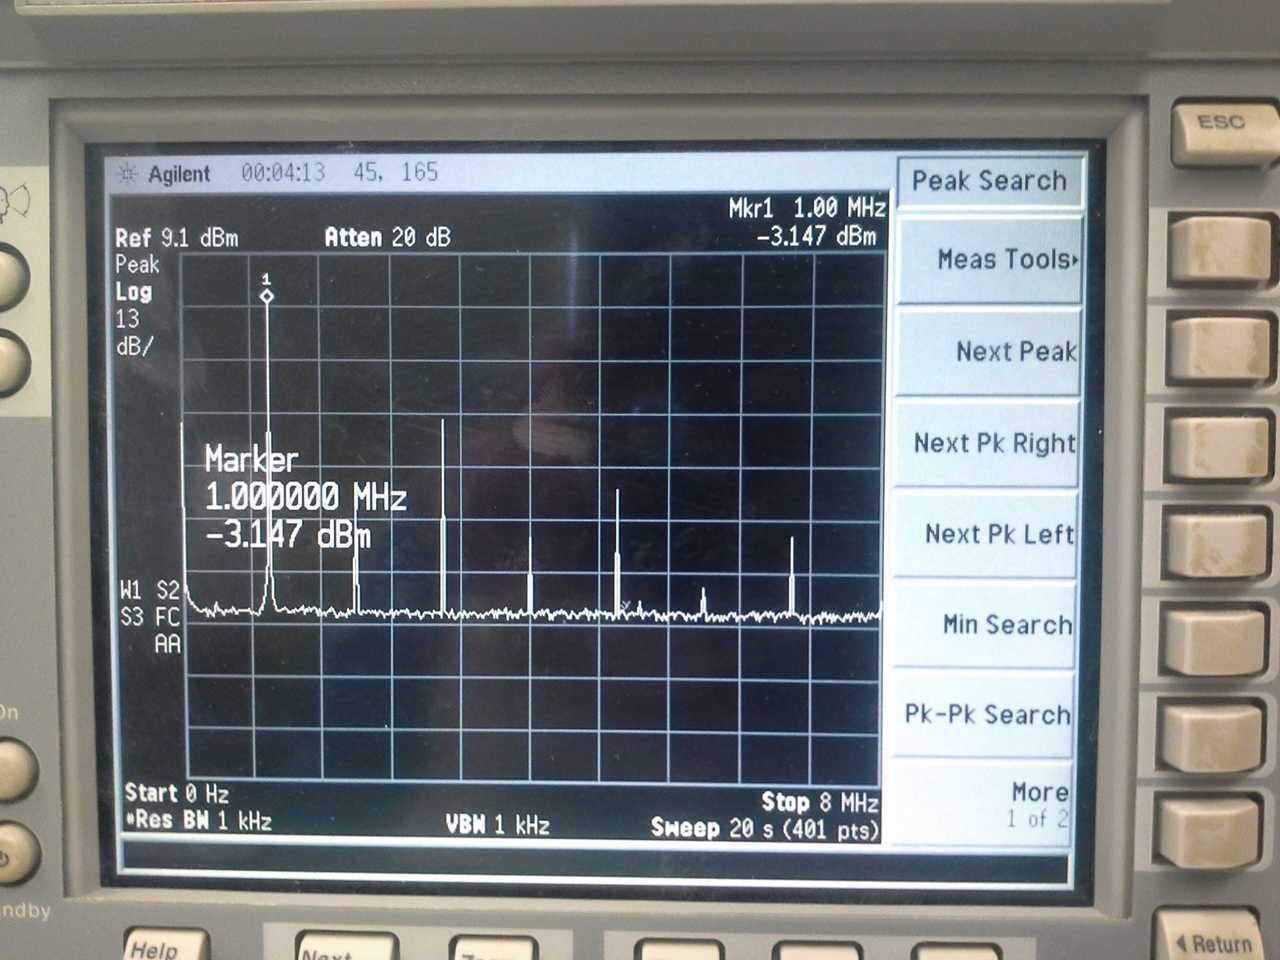
\includegraphics[scale=0.17]{../Grafiken/TraegerspannungOberwellen_0.jpg}
	\caption{Grundschwingung \label{fig:traegerspannungoberwellen_0}}
\end{subfigure}%
~
\begin{subfigure}[t]{0.5\textwidth}
	\centering
	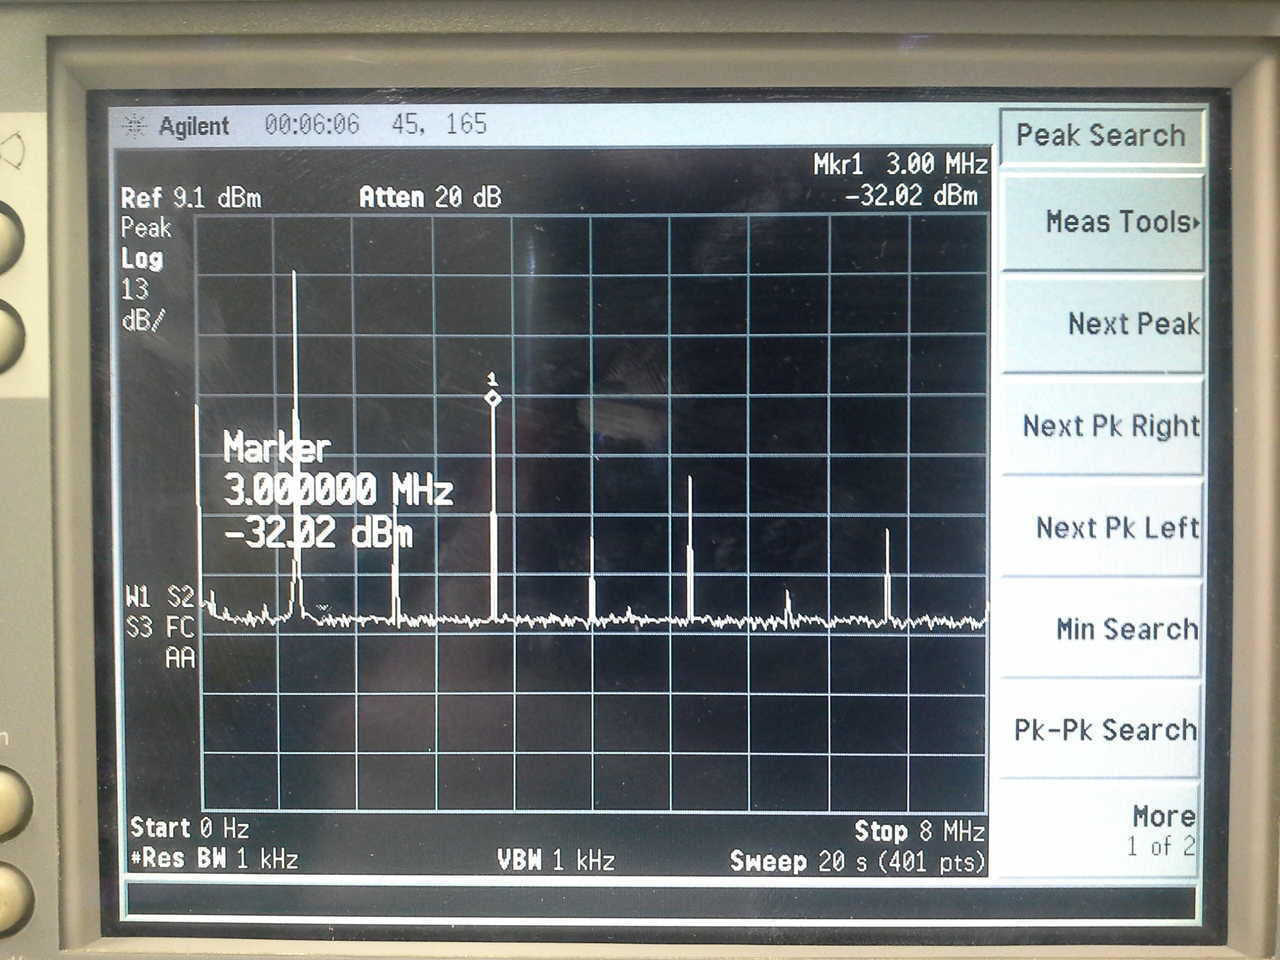
\includegraphics[scale=0.17]{../Grafiken/TraegerspannungOberwellen_2.jpg}
	\caption{Zweite Oberschwingung\label{fig:traegerspannungoberwellen_2}}
\end{subfigure}
	\caption{Frequenzspektrum der verwendeten Trägerspannung. Zu erkennen sind die Oberschwingungen,
		     die bereits in der ursprünglichen Spannung vorhanden sind. \label{fig:traegerspannungoberwellen}}
\end{figure}
\FloatBarrier

\FloatBarrier
\begin{figure}[!h]
\begin{subfigure}[t]{0.5\textwidth}
	\centering
	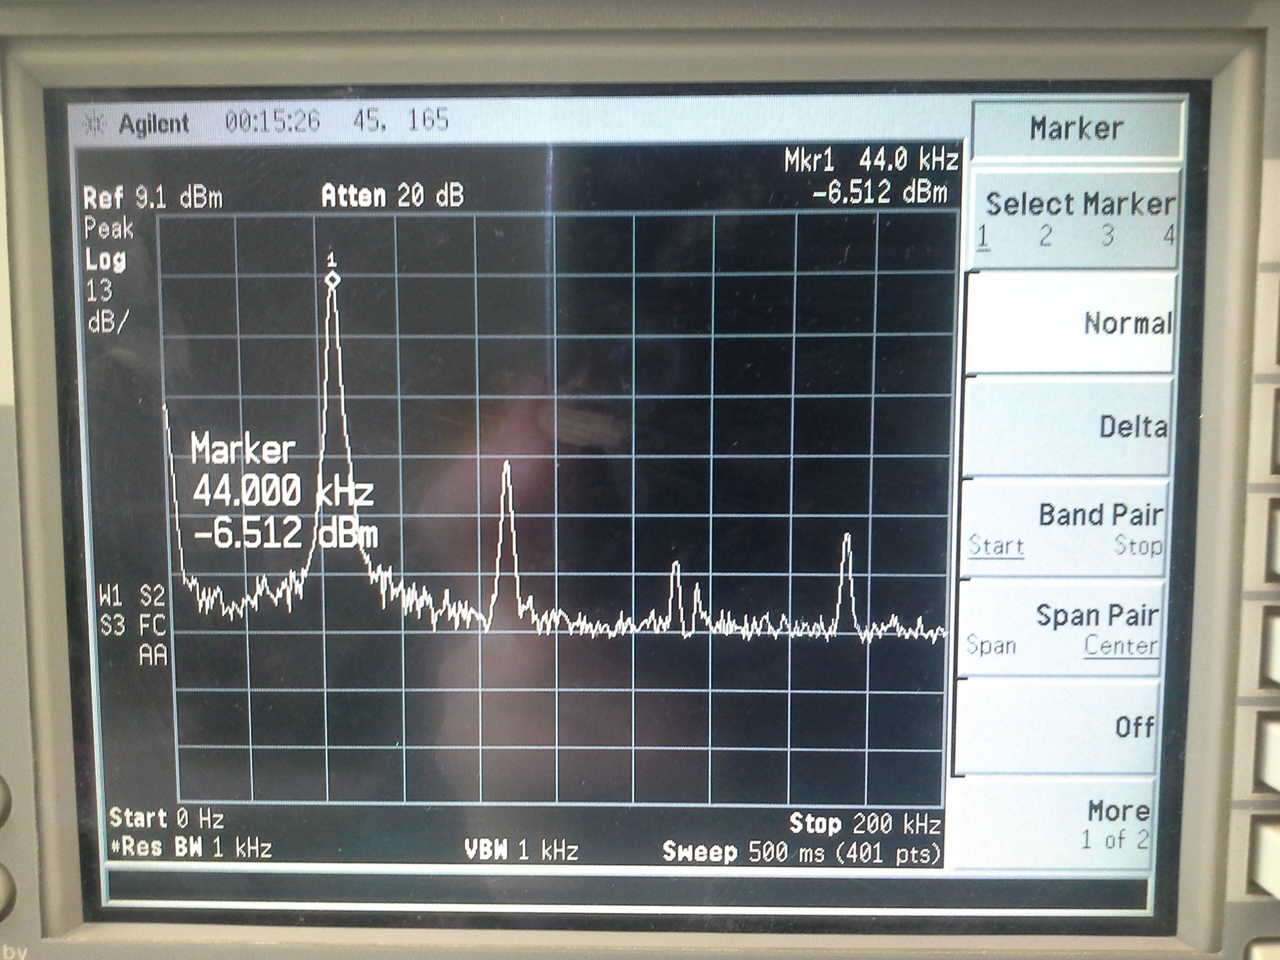
\includegraphics[scale=0.17]{../Grafiken/ModulationsspannungOberwellen_0.jpg}
	\caption{Grundschwingung \label{fig:modulationsspannungoberwellen_0}}
\end{subfigure}%
~
\begin{subfigure}[t]{0.5\textwidth}
	\centering
	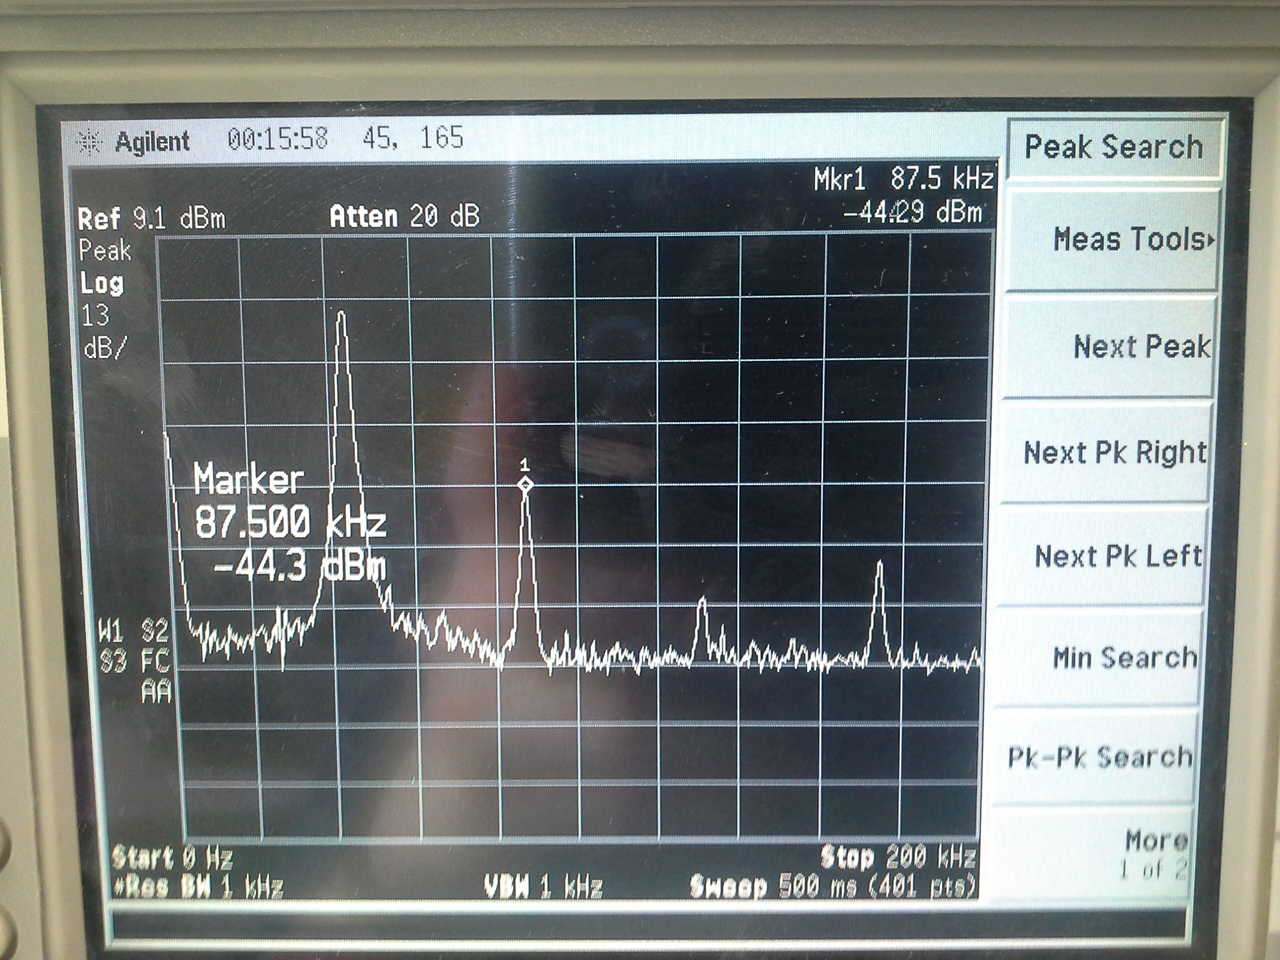
\includegraphics[scale=0.17]{../Grafiken/ModulationsspannungOberwellen_1.jpg}
	\caption{Erste Oberschwingung\label{fig:modulationsspannungoberwellen_1}}
\end{subfigure}
	\caption{Frequenzspektrum der verwendeten Modulationsspannung. Zu erkennen sind die Oberschwingungen,
		     die bereits in der ursprünglichen Spannung vorhanden sind. \label{fig:modulationsspannungoberwellen}}
\end{figure}
\FloatBarrier

An diesen Spektren ist zu erkennen, dass bereits die von den Generatoren erzeugten Spannungen mehr 
als nur eine Frequenz enthalten. Es ist somit davon auszugehen, dass durch diese Störterme verursacht
werden, die die Qualität der durchgeführten Modulationen negativ beeinflussen. 

\subsection{Amplitudenmodulation von Spannungen}

Die unter Verwendung des Ringmodulators erzeugte, amplitudenmodulierte Spannung mit Trägerunterdrückung 
ist in \cref{fig:amplituden_modulierte_spannung_ohne_traeger} dargestellt. Für die Erzeugung dieser Spannung
wurden die folgenden Werte für Amplitude $\hat{U}$ und Frequenz $f$ der Träger- und Modulationsspannung
eingestellt.
\begin{empheq}{alignat=3}
	\label{eq:ausgangswerte_ohne_traeger}
	\hat{U}_{\text{T}} &= \SI{968(1)}{\milli\volt} \quad
	f_{\text{T}} \,&= \, &\SI{1.000(1)}{\mega\hertz} \\
	\hat{U}_{\text{M}} &= \SI{301(1)}{\milli\volt} \quad \notag
	f_{\text{M}} \,&=\, &\SI{43(1)}{\kilo\hertz}
\end{empheq}
 
Nach \cref{eq:amplituden_moduliert_ohne_traeger} hat eine auf diese Art modulierte Spannung die Gestalt einer
Schwebung, welche in der angegebene Abbildung zu erkennen ist.


\FloatBarrier\begin{figure}[!h]
\centering
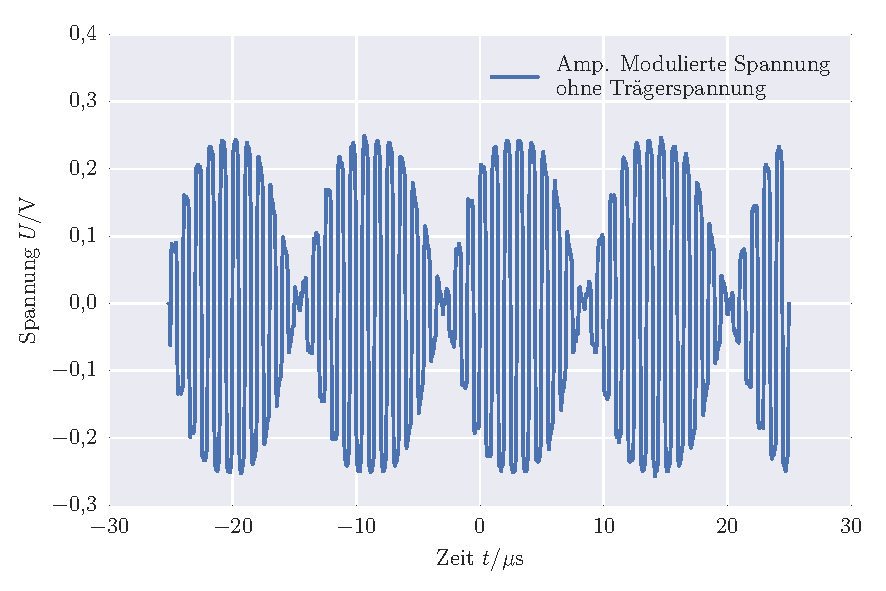
\includegraphics[scale=1]{../Grafiken/Amplituden_Modulierte_Spannung_ohne_Traeger.pdf}
\caption{Ergebnisspannung der Amplitudenmodulation mit Trägerunterdrückung. \label{fig:amplituden_modulierte_spannung_ohne_traeger}}
\end{figure}
\FloatBarrier

In der \cref{fig:frequenzspektrum_b_ampmodulierttraegerunterdrueckung} ist das Spektrum dieser
amplitudenmodulierten Spannung dargestellt. In \cref{fig:frequenzspektrum_b_ampmodulierttraegerunterdrueckung_0}
ist die trotz Trägerunterdrückung vorhandene Trägerspannung und in 
\cref{fig:frequenzspektrum_b_ampmodulierttraegerunterdrueckung_1} der Frequenzunterschied der ersten beiden 
Seitenbänder hervorgehoben. 

\FloatBarrier
\begin{figure}
	\begin{subfigure}[t]{0.5\textwidth}
		\centering
		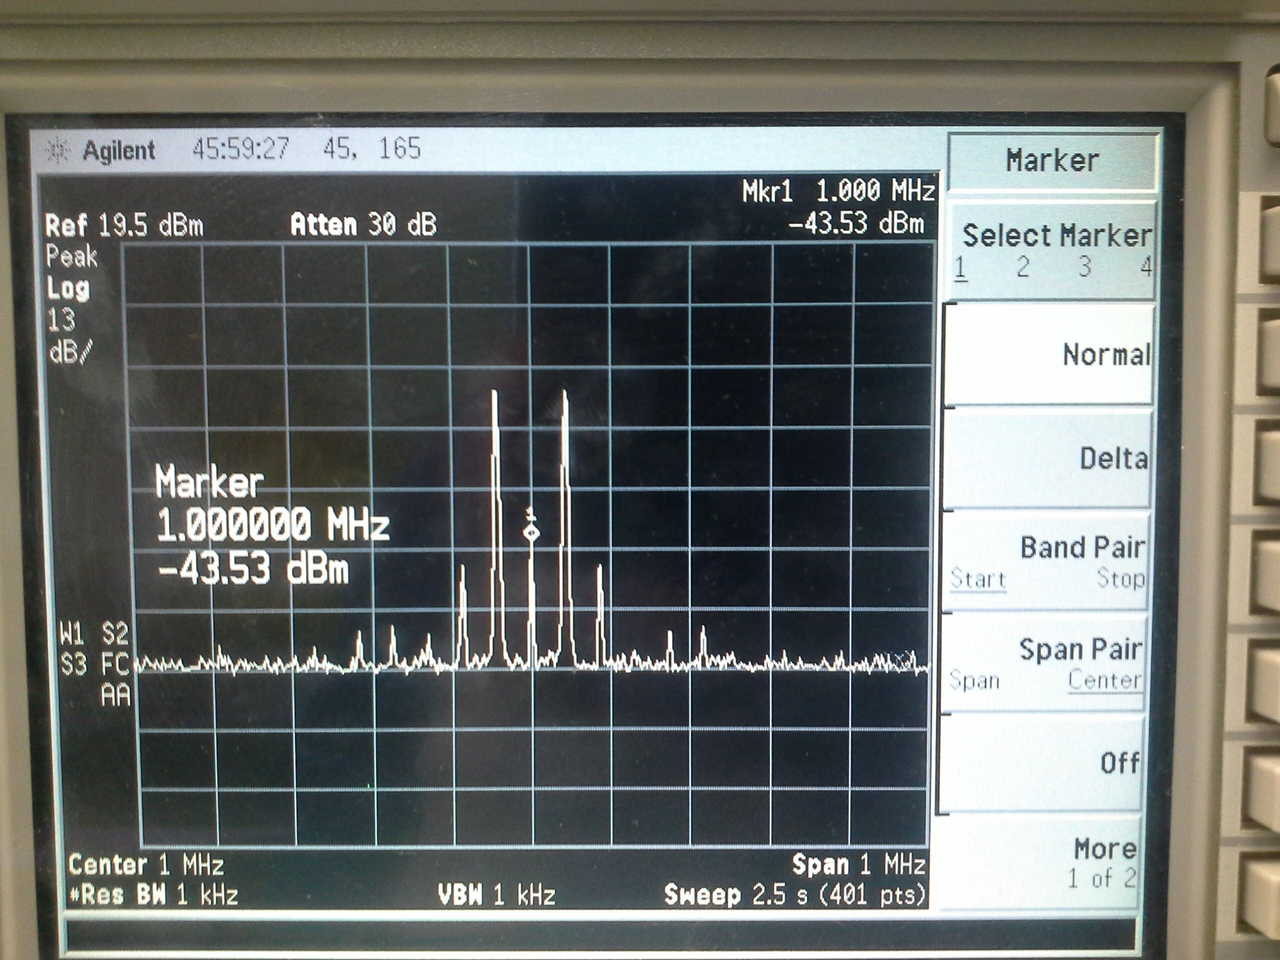
\includegraphics[scale=0.17]{../Grafiken/Frequenzspektrum_b_AmpModuliertTraegerunterdrueckung_0.jpg}
		\caption{Trägerfrequenz\label{fig:frequenzspektrum_b_ampmodulierttraegerunterdrueckung_0}}
	\end{subfigure}%
	~
	\begin{subfigure}[t]{0.5\textwidth}
		\centering
		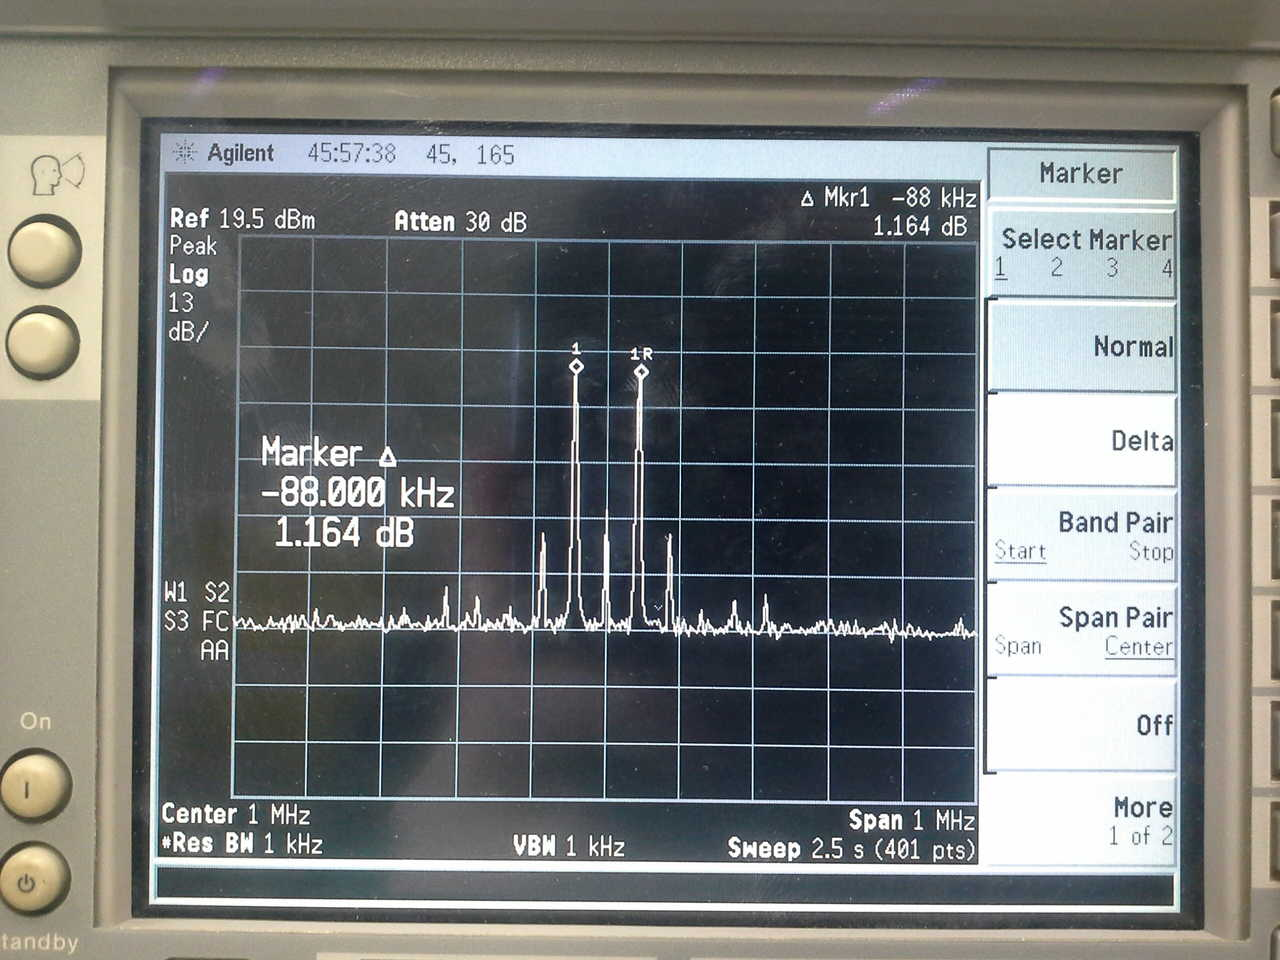
\includegraphics[scale=0.17]{../Grafiken/Frequenzspektrum_b_AmpModuliertTraegerunterdrueckung_1.jpg}
		\caption{Frequenzunterschied der Seitenbänder \label{fig:frequenzspektrum_b_ampmodulierttraegerunterdrueckung_1}}
	\end{subfigure}
	\caption{Frequenzspektrum der amplitudenmodulierten Spannung mit Trägerunterdrückung. Dargestellt ist 
		die Trägerfrequenz (a) und der Frequenzunterschied der ersten beiden Seitenbänder (b).
		\label{fig:frequenzspektrum_b_ampmodulierttraegerunterdrueckung}}
\end{figure}
\FloatBarrier

Das Auftreten der stark gedämpften Trägerfrequenz ist dabei auf eine nicht 
ideale Multiplikation der Spannungen durch den Ringmodulator zurückzuführen. 
Anhand des dargestellten Frequenzunterschieds zeigt sich, dass die beiden Seitenbänder bei den erwarteten 
Frequenzen $f_{\text{T}} \pm f_{\text{M}}$ liegen.


Die Amplitudenmodulation mit Trägerabstrahlung, die mit Hilfe einer Germanium-Diode durchgeführt wurde 
lieferte die in \cref{fig:amplituden_modulierte_spannung_mit_traeger} gezeigte Spannung.
Für die Erzeugung wurden die folgenden Werte der Ausgangsspannungen verwendet.

\begin{empheq}{alignat=3}
\label{eq:ausgangswerte_mit_traeger}
\hat{U}_{\text{T}} &= \SI{938(1)}{\milli\volt} \quad
f_{\text{T}} \,&=\, &\SI{1.988(1)}{\mega\hertz} \\
\hat{U}_{\text{M}} &= \SI{100(1)}{\milli\volt} \notag \quad 
f_{\text{M}} \,&=\, &\SI{94(1)}{\kilo\hertz}
\end{empheq} 



\FloatBarrier\begin{figure}[!h]
\centering
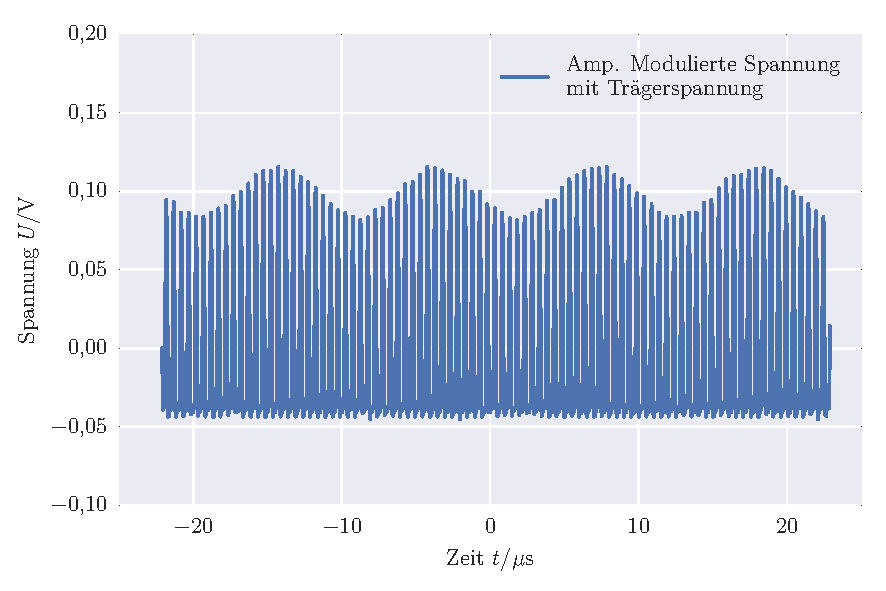
\includegraphics[scale=1]{../Grafiken/Amplituden_Modulierte_Spannung_mit_Traeger.pdf}
\caption{\label{fig:amplituden_modulierte_spannung_mit_traeger}}
\end{figure}
\FloatBarrier

Die Verwendung einer Diode führt dazu, dass die unteren Halbwellen der Spannung abgeschnitten werden, 
sodass die Modulation nur noch an der Variation der Amplitude der oberen Halbwellen erkennbar ist.
Für die Bestimmung des Modulationsgrades $m$ aus der Zeitabhängigkeit der modulierten Spannung
wurden diese Amplituden in \cref{fig:amplituden_modulierte_spannung_mit_traeger_modulationsgrad}
einzeln dargestellt. Ferner wurden jeweils die lokalen Extrema der Amplitude hervorgehoben und
aus diesen Werten jeweils der Mittelwert für Minimum und Maximum zu
\begin{empheq}{align*}
	\mean{\hat{U}_{\text{min}}} &= \SI{0.083(1)}{\volt}\\
	\mean{\hat{U}_{\text{max}}} &= \SI{0.1154(4)}{\volt},
\end{empheq}
bestimmt. Nach den in \cref{fig:modulationsgrad_amplitude}
dargestellten Gleichungen und den hier bestimmten Werten folgt für den Modulationsgrad
\begin{empheq}{equation}
	m = \frac{\mean{\hat{U}_{\text{max}}} - \mean{\hat{U}_{\text{min}}}}{\mean{\hat{U}_{\text{max}}} + \mean{\hat{U}_{\text{min}}}} = \num{0.164(6)}.
\end{empheq}  


%U_min = 0.0829+/-0.0010
%U_max = 0.1154+/-0.0004ein
%m = 0.164+/-0.006


\FloatBarrier\begin{figure}[!h]
\centering
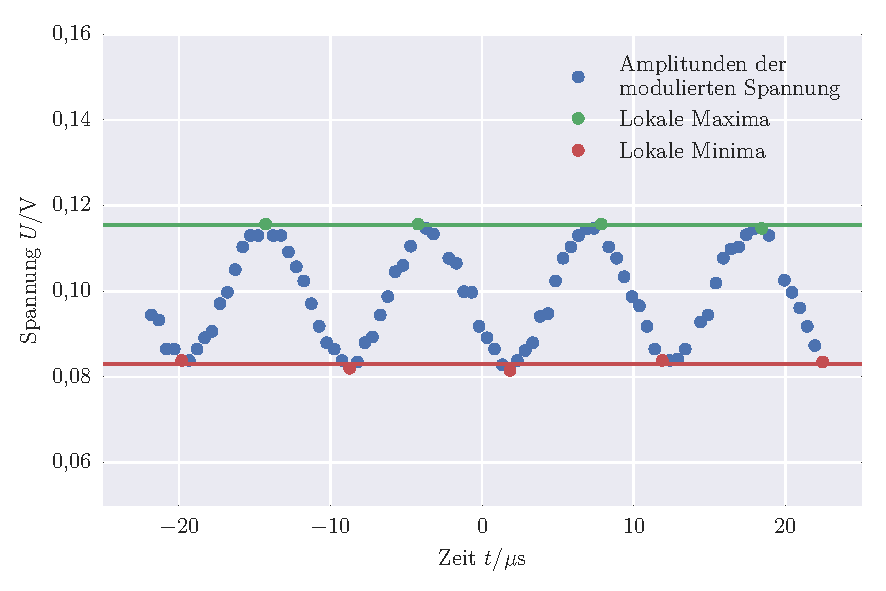
\includegraphics[scale=1]{../Grafiken/Amplituden_Modulierte_Spannung_mit_Traeger_Modulationsgrad.pdf}
\caption{Amplituden der amplitudenmodulierten Spannung aus \cref{fig:amplituden_modulierte_spannung_mit_traeger}.
Farblich hervorgehoben sind jeweils die lokalen Extrema. Die abgebildet Geraden markieren jeweils den Mittelwert
dieser Extremwerte.
 \label{fig:amplituden_modulierte_spannung_mit_traeger_modulationsgrad}}
\end{figure}
\FloatBarrier

Das Frequenzspektrum der modulierten Spannung ist in \cref{fig:frequenzspektrum_c_ampmodulierttraeger}
gezeigt. Aus \cref{fig:frequenzspektrum_c_ampmodulierttraeger_differenz} ist erkennbar, dass die 
Seitenbänder der Modulation wie zuvor bei den erwarteten Frequenzen 
$f_{\text{T}} \pm f_{\text{M}}$ liegen. Aus den Abbildungen \ref{fig:frequenzspektrum_c_ampmodulierttraeger_oberwellen_0}  und \ref{fig:frequenzspektrum_c_ampmodulierttraeger_oberwellen_1} wird ersichtlich, dass wegen 
der nicht linearen Kennlinie der Diode mit der die Modulation durchgeführt wurde Oberschwingungen 
der Trägerfrequenz auftreten. Ein zusätzlicher Beitrag stammt von den Oberschwingungen die bereits in den 
Ausgangsspannungen vorhanden waren.  
 

\FloatBarrier\begin{figure}[!h]
\centering
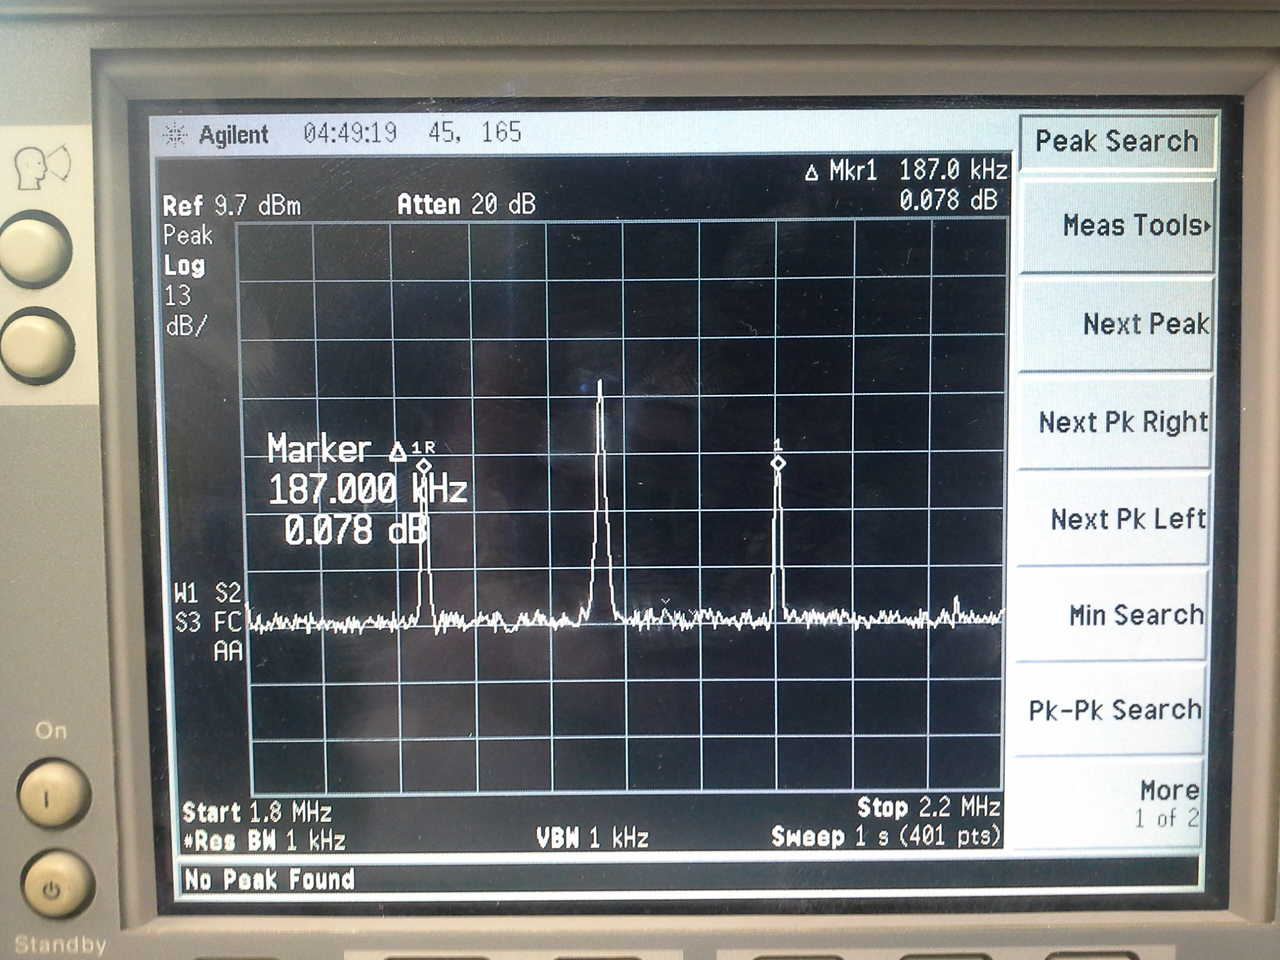
\includegraphics[scale=1]{../Grafiken/Frequenzspektrum_c_AmpModuliertTraeger.jpg}
\caption{\label{fig:frequenzspektrum_c_ampmodulierttraeger}}
\end{figure}
\FloatBarrier

Für die Bestimmung des Modulationsgrad aus dem Spektrum werden die Amplituden der Grundschwingung \ref{fig:frequenzspektrum_c_ampmodulierttraeger_oberwellen_0} und die Amplitude der Seitenbänder 
\ref{fig:frequenzspektrum_c_ampmodulierttraeger} benötigt. 
Der Leistungspegel der Grundschwingung ist mit $L_{\text{P,T}}= \SI{-25.56}{dBm}$ angeben. Aus der Einteilung der
$y$-Richtung des Frequenzanalysators (\SI{13}{dB/}) lässt sich der Leistungspegel der Seitenbänder 
durch nachmessen auf $L_{\text{P,T$\pm$M}}= \SI{-46.56}{dBm}$ bestimmen.
Der Leistungspegel gibt das logarithmierte Verhältnis der Leistung zu $P_{0} = \SI{1}{\milli\watt}$ an.
Damit folgt für die Leistung,
\begin{empheq}{equation}
	P = 10^{\frac{L_{p}}{10}} \cdot P_{0}.
\end{empheq}
Die Leistung ist nun proportional zum Quadrat der Amplitude der Spannung, sodass
sich für die gesuchten Amplituden,
\begin{empheq}{align*}
\hat{U}_{\text{T}} &\propto \SI{0.053}{\volt}\\
\hat{U}_{\text{T$\pm$M}} &\propto \SI{0.005}{\volt},
\end{empheq}
ergibt. Aus der \cref{fig:Frequenzspektrum} und den berechneten Werten folgt für den Modulationsgrad
\begin{empheq}{equation}
m = \frac{2\cdot\hat{U}_{\text{T$\pm$M}}}{\hat{U}_{\text{T}}}= \num{0.178}.
\label{eq:modulationsgrad_frequenz}
\end{empheq} 
Diese Berechnung kann durchgeführt werden, da die Proportionalitätskonstante für die Spannungen jeweils
die gleiche ist, sodass diese sich bei der Division der Spannungen kürzt.   

Wird die Berechnung nach \cref{eq:modulationsgrad_frequenz} mit den Einstellungen 
\eqref{eq:ausgangswerte_mit_traeger} durchgeführt so ergibt sich ein Modulationsgrad von 
$m = \num{0.213}$, welcher in der gleichen Größenordnung wie die zuvor bestimmten Werte liegt. 

%Spannung(Träger): 0.0527229861423 V
%Spannung(Modulation): 0.00469894108605 V
%Modulationsgrad: 0.178250187627

\subsection{Demodulation von Amplitudenmodulierten Spannungen}

Vor der Verwendung des Ringmodulators für die Demodulation einer amplitudenmodulierten Spannung.
soll zunächst die Abhängigkeit der Gleichspannung am Ausgang X des Ringmodulators von der Phase
$\varphi$ zwischen den Wechselspannungen an den Eingängen R und L betrachtet werden. Die 
zu diesem Zweck aufgenommenen Messwerte sind \cref{tab:messwerte_phasenempfindlicher_gleichrichter} 
abzulesen und in \cref{fig:phasenempfindlicher_gleichrichter} 
mit entsprechender Ausgleichskurve der Gestalt
\begin{empheq}{equation}
	U(\varphi) = a \cdot cos(\varphi + b), 
\end{empheq}
aufgetragen. Die Ausgleichsrechnung ergab die Parameter
\addtocounter{equation}{-1}
\begin{subequations}
\begin{empheq}{align}
	a &= \SI{89(2)}{\milli\volt}\\
	b &= \SI{0.05(2)}{rad} = \SI{3(1)}{\degree}.
\end{empheq}
\end{subequations}

\begin{table}[!h]
	\centering
	\begin{tabular}{cccccc}
		\toprule
		Frequenz & Spannung & Phase & Frequenz & Spannung & Phase\\
		$f$/\si{\kilo\hertz} & $U$/\si{\milli\volt} & $\varphi$/\si{rad} & $f$/\si{\kilo\hertz} & $U$/\si{\milli\volt} & $\varphi$/\si{rad}\\
\midrule
		\num{252(1)} & \num{70(1)} & \num{0.396(2)} & \num{2250(1)} & \num{-83(1)} & \num{3.534(2)}\\
		\num{500(1)} & \num{56(1)} & \num{0.785(2)} & \num{2499(1)} & \num{-62(1)} & \num{3.925(2)}\\
		\num{750(1)} & \num{28(1)} & \num{1.178(2)} & \num{2750(1)} & \num{-31(1)} & \num{4.320(2)}\\
		\num{1000(1)} & \num{-4(1)} & \num{1.571(2)} & \num{3008(1)} & \num{3(1)} & \num{4.725(2)}\\
		\num{1251(1)} & \num{-37(1)} & \num{1.965(2)} & \num{3252(1)} & \num{36(1)} & \num{5.108(2)}\\
		\num{1505(1)} & \num{-65(1)} & \num{2.364(2)} & \num{3496(1)} & \num{66(1)} & \num{5.492(2)}\\
		\num{1746(1)} & \num{-80(1)} & \num{2.743(2)} & \num{3753(1)} & \num{89(1)} & \num{5.897(2)}\\
		\num{2001(1)} & \num{-85(1)} & \num{3.145(2)} & \num{4002(1)} & \num{98(1)} & \num{6.286(2)}\\
		\bottomrule
	\end{tabular}
	\caption{In Abhängigkeit der Frequenz der Eingangssignale gemessene Ausgangsspannung an dem verwendeten Ringmodulator.
             Durch die Verwendung einer Leitung mit der festen Laufzeit von $\Delta t = \SI{250}{\nano\metre}$ ist die eingestellte
             Frequenz proportional zu der Phase zwischen den beiden Eingangsspannungen. 
             Diese wurde über $\varphi = 2\pi f \Delta t$ bestimmt. \label{tab:messwerte_phasenempfindlicher_gleichrichter}}
\end{table}


Die Abbildung und die geringe Phasenverschiebung der Ausgleichskurve, 
zeigt eine Übereinstimmung mit dem erwarteten Zusammenhang, mit nur 
geringen Abweichungen. 

%Amplitude: 89.1+/-1.6
%Phase: 0.048+/-0.018 2.8+/-1.0


\FloatBarrier\begin{figure}[!h]
\centering
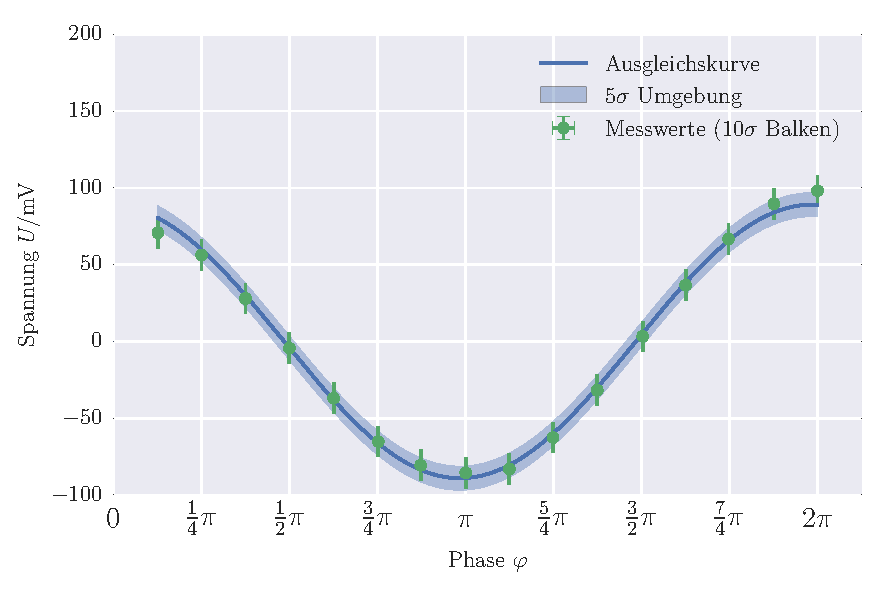
\includegraphics[scale=1]{../Grafiken/Phasenempfindlicher_Gleichrichter.pdf}
\caption{Darstellung der Abhängigkeit der Ausgangs-Gleichspannung des 
	Ringmodulators von der Phase $\varphi$ der Eingangs-Wechselspannungen. 
	Die Fehler der Messwerte sind aufgrund ihres geringen Wertes verzehnfacht
	dargestellt. Und auch das Fehlerband der Ausgleichskurve wurde mit fünf skaliert,
	um sichtbar zu sein.
	\label{fig:phasenempfindlicher_gleichrichter}}
\end{figure}
\FloatBarrier

Die Demodulation einer amplitudenmodulierten Spannung\footnote{Unter Verwendung der Einstellungen 
\eqref{eq:ausgangswerte_ohne_traeger} erzeugt.} mit der Ringmodulatorschaltung
liefert die in \cref{fig:amplituden_modulation_ring_demodulation} dargestellte Spannung.
Zum Vergleich ist zusätzlich die ursprüngliche Modulationsspannung dargestellt. 
Es zeigt sich, dass die beiden Spannungen in ihrer Zeitabhängigkeit sehr ähnlich sind, jedoch tritt zwischen 
Modulationsspannung und der demodulierter Spannung eine Phase auf. Diese lässt sich durch die unterschiedlichen
Laufzeiten der Spannungen in den verwendeten Kabeln erklären, die sowohl von der Frequenz der Spannung als auch 
von der Länge der Kabel selbst abhängt. 


\FloatBarrier\begin{figure}[!h]
\centering
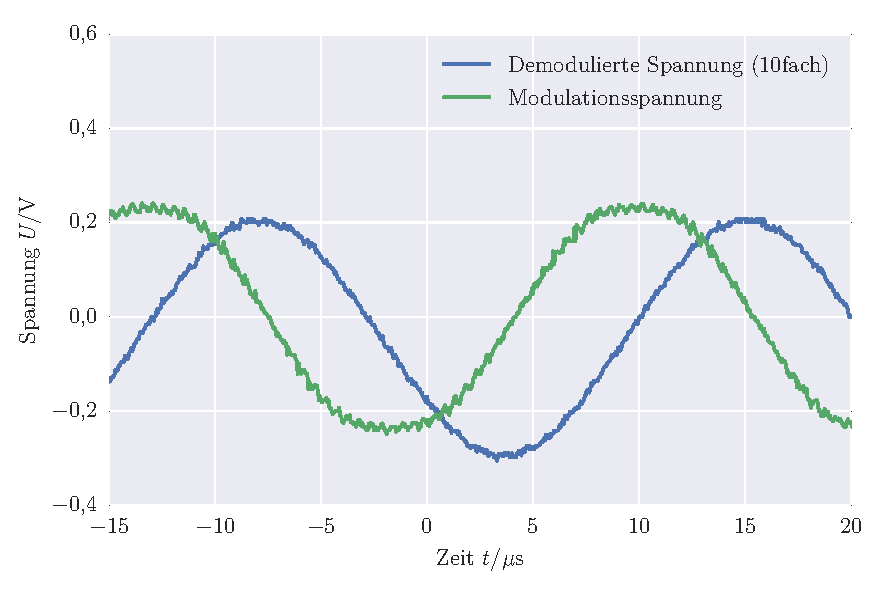
\includegraphics[scale=1]{../Grafiken/Amplituden_Modulation_Ring_Demodulation.pdf}
\caption{\label{fig:amplituden_modulation_ring_demodulation}}
\end{figure}
\FloatBarrier

Die Demodulation der amplitudenmodulierten Spannung\footnotemark[1] %\footnote{Unter Verwendung der Einstellungen 
%	\eqref{eq:ausgangswerte_ohne_traeger} erzeugt.} 
mit einer Diode liefert
nach der Diode die in \cref{fig:amplituden_modulation_diode_demodulation_gleichrichter}
dargestellte Spannung. Die Spannung an dem nachgeschalteten Tiefpass kann in 
\cref{fig:amplituden_modulation_diode_demodulation_tiefpass} betrachtet werden.
Der Spannungsverlauf nach der Diode zeigt, wie zu erwarten ist, dass die unteren Halbwellen 
durch die Diode unterdrückt werden. Im Vergleich zur Modulationsspannung zeigt sich
ferner, dass die Amplitude der übrigen Halbwellen mit der Modulationsfrequenz variiert.
Der nachgeschaltete Tiefpass wird nun dazu verwendet,
die Frequenzen oberhalb der Modulationsfrequenz zu unterdrücken, sodass man diese 
lediglich Phasenverschoben und in diesem Fall stark abgeschwächt zurückerhält.
Die Abschwächung ist dabei auf die Widerstände in den verwendeten Schaltungen zurückzuführen.


\FloatBarrier
\begin{figure}[!h]
\centering
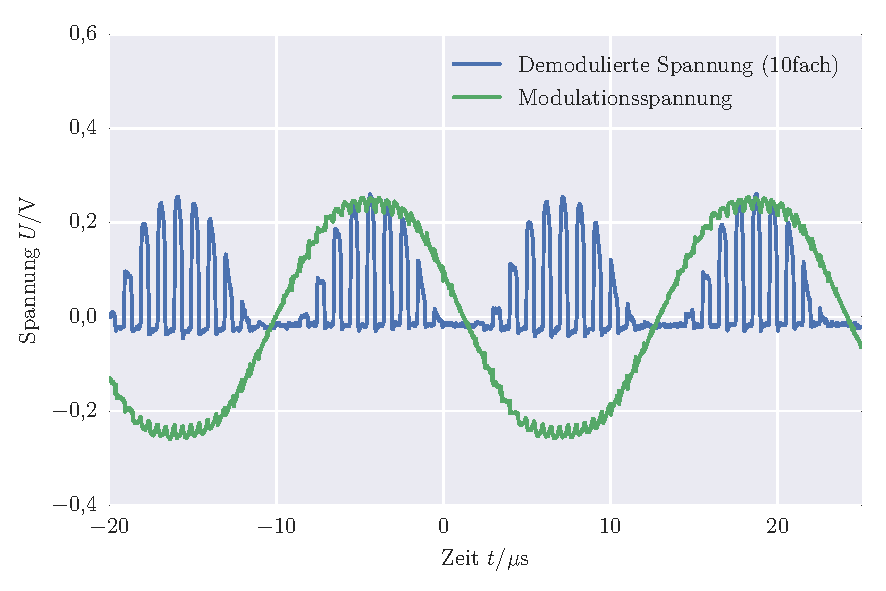
\includegraphics[scale=1]{../Grafiken/Amplituden_Modulation_Diode_Demodulation_Gleichrichter.pdf}
\caption{Spannung die in der Demodulationsschaltung mit Diode nach ebendieser abgegriffen wurde.
	Zu erkennen ist, dass die unteren Halbwellen der modulierten Eingangsspannung durch die Diode
	unterdrückt werden. Der Vergleich mit der Modulationsspannung zeigt das die übrig gebliebenen 
	oberen Halbwellen ihre Amplitude mit der Modulationsfrequenz verändern.   
	\label{fig:amplituden_modulation_diode_demodulation_gleichrichter}}
\end{figure}
\FloatBarrier


\FloatBarrier\begin{figure}[!h]
\centering
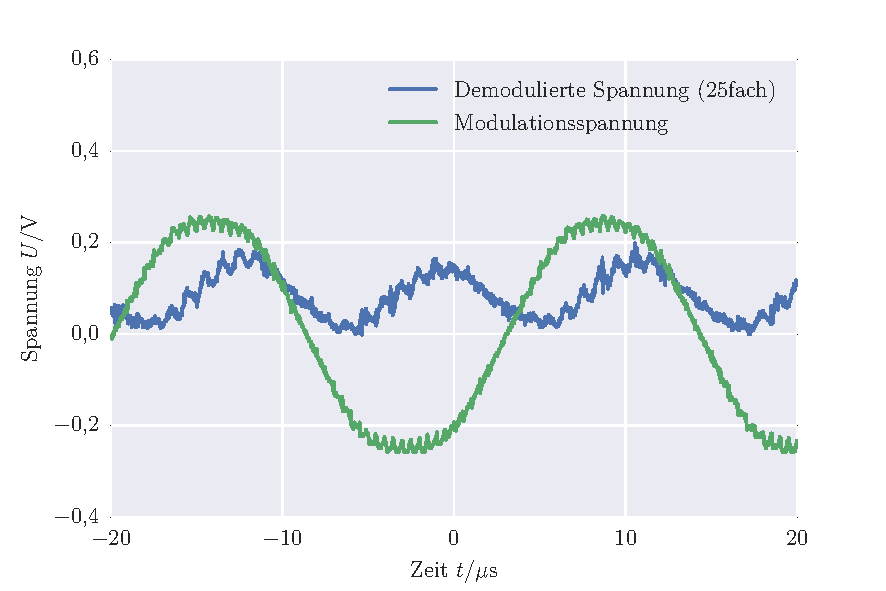
\includegraphics[scale=1]{../Grafiken/Amplituden_Modulation_Diode_Demodulation_Tiefpass.pdf}
\caption{Ergebnisspannung nach Demodulation mit einer Diode und Unterdrückung höherer Frequenzen mit 
	einem Tiefpass. Im Vergleich zur Modulationsfrequenz wird ersichtlich, dass man diese nach der
	Demodulation in abgeschwächter Form und Phasenverschoben zurückerhält.
	  \label{fig:amplituden_modulation_diode_demodulation_tiefpass}}
\end{figure}
\FloatBarrier



\subsection{Frequenzmodulation von Spannungen}\label{sec:Frequenzmodulation}

Für die Frequenzmodulation der Trägerspannung werden nach \cref{eq:frequenzmodulation} die beiden Seitenbänder einer 
Amplitudenmodulation (mit einem Ringmodulator) und die 
um $\tfrac{\pi}{2}$ phasenverschobene Trägerspannung benötigt.
Für die Spannungen wurden die folgenden Einstellungen verwendet.
\begin{empheq}{alignat=3}
\label{eq:ausgangswerte_frequenz}
\hat{U}_{\text{T}} &= \SI{969(1)}{\milli\volt} \quad
f_{\text{T}} \,&=\, &\SI{1.000(1)}{\mega\hertz} \\
 \notag
\hat{U}_{\text{M}} &= \SI{580(1)}{\milli\volt} \quad
f_{\text{M}} \,&=\, &\SI{43(1)}{\kilo\hertz}
\end{empheq} 

In \cref{fig:frequenz_modulierte_spannung} ist die entsprechende Ergebnisspannung 
dargestellt. Die Frequenzvariation ist, trotz des geringen Maßes, an den Abständen 
der Nulldurchgänge der Spannung zu erkennen. Desweiteren lässt sich ebenfalls eine 
geringe Variation in der Amplitude feststellen. Dies lässt darauf schließen, dass 
die Phasenverschiebung nicht exakt um $\tfrac{\pi}{2}$ durchgeführt wurde.
Dies führt aufgrund des trigonometrischen Additionstheorems
\begin{empheq}{equation}
	\cos(\omega t \pm \varphi) = \cos(\omega t)\cos(\varphi) \mp \sin(\omega t)\sin(\varphi)
\end{empheq}
zu nicht verschwindenden Kosinusanteilen und damit zu einem geringen Maß an Amplitudenmodulation.


\FloatBarrier\begin{figure}[!h]
\centering
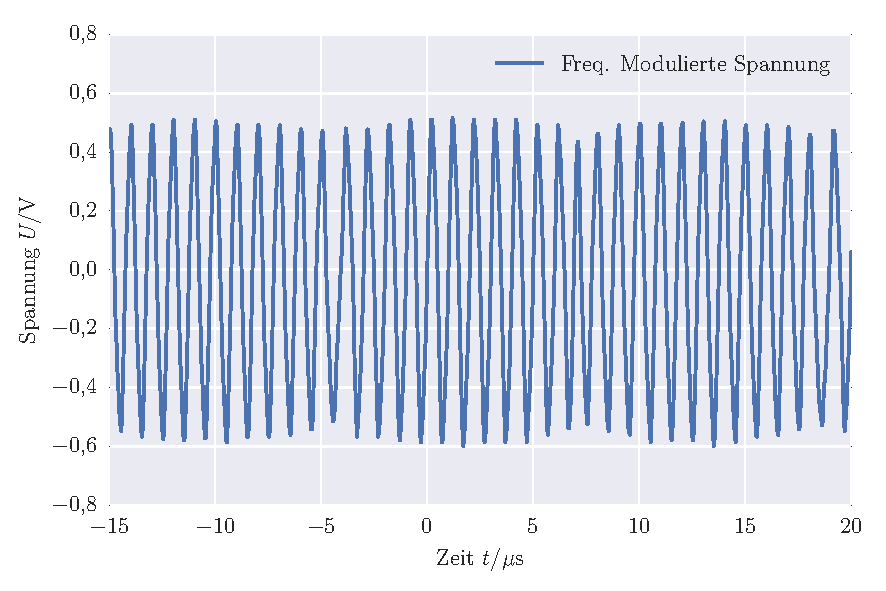
\includegraphics[scale=1]{../Grafiken/Frequenz_Modulierte_Spannung.pdf}
\caption{Frequenzmodulierte Spannung die durch Addition der Seitenbänder aus einer Amplitudenmodulation
	mit Trägerunterdrückung und der phasenverschobenen Trägerspannung erzeugt wurde. Neben der schwachen 
	Frequenzmodulation ist zusätzlich eine geringe Amplitudenmodulation festzustellen.  \label{fig:frequenz_modulierte_spannung}}
\end{figure}
\FloatBarrier

In \cref{fig:frequenzspektrum_d_freqmoduliert} ist das Frequenzspektrum dieser
frequenzmodulierten Spannung dargestellt. In \cref{fig:frequenzspektrum_d_freqmoduliert_0}
ist die Trägerfrequenz hervorgehoben, während die Abbildungen \ref{fig:frequenzspektrum_d_freqmoduliert_1}
und \ref{fig:frequenzspektrum_d_freqmoduliert_2} die Frequenzunterschiede der ersten und zweiten Seitenbänder 
aufzeigen. Aus diesen Abbildungen ist ersichtlich, dass die Seitenbänder bei den erwarteten Frequenzen
$f_{\text{T}} \pm nf_{\text{M}}$ liegen. Da nicht nur die erste Ordnung an Seitenbändern auftritt,
ist außerdem festzustellen, dass die Frequenzmodulation keinen geringen Frequenzhub besitzt. Neben dieser
Ursache tragen auch die Oberschwingungen in den verwendeten Eingangsspannungen zum Auftreten dieser Frequenzen
bei.   
\FloatBarrier
\begin{figure}[!h]
	\begin{subfigure}[t]{1\textwidth}
		\centering
		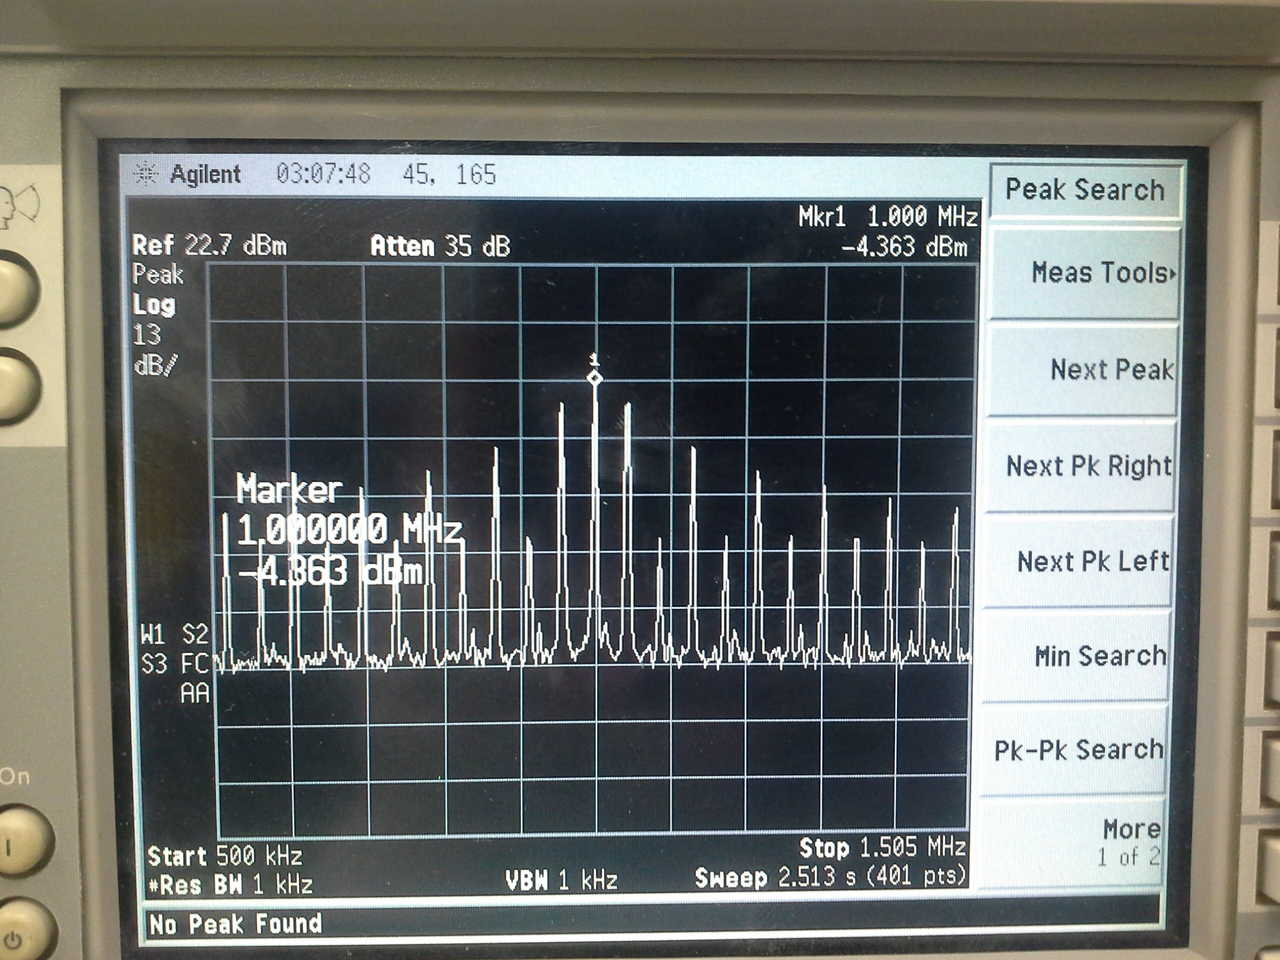
\includegraphics[scale=0.17]{../Grafiken/Frequenzspektrum_d_FreqModuliert_0.jpg}
		\caption{Grundfrequenz\label{fig:frequenzspektrum_d_freqmoduliert_0}}
	\end{subfigure}%
	
	\begin{subfigure}[t]{0.5\textwidth}
		\centering
		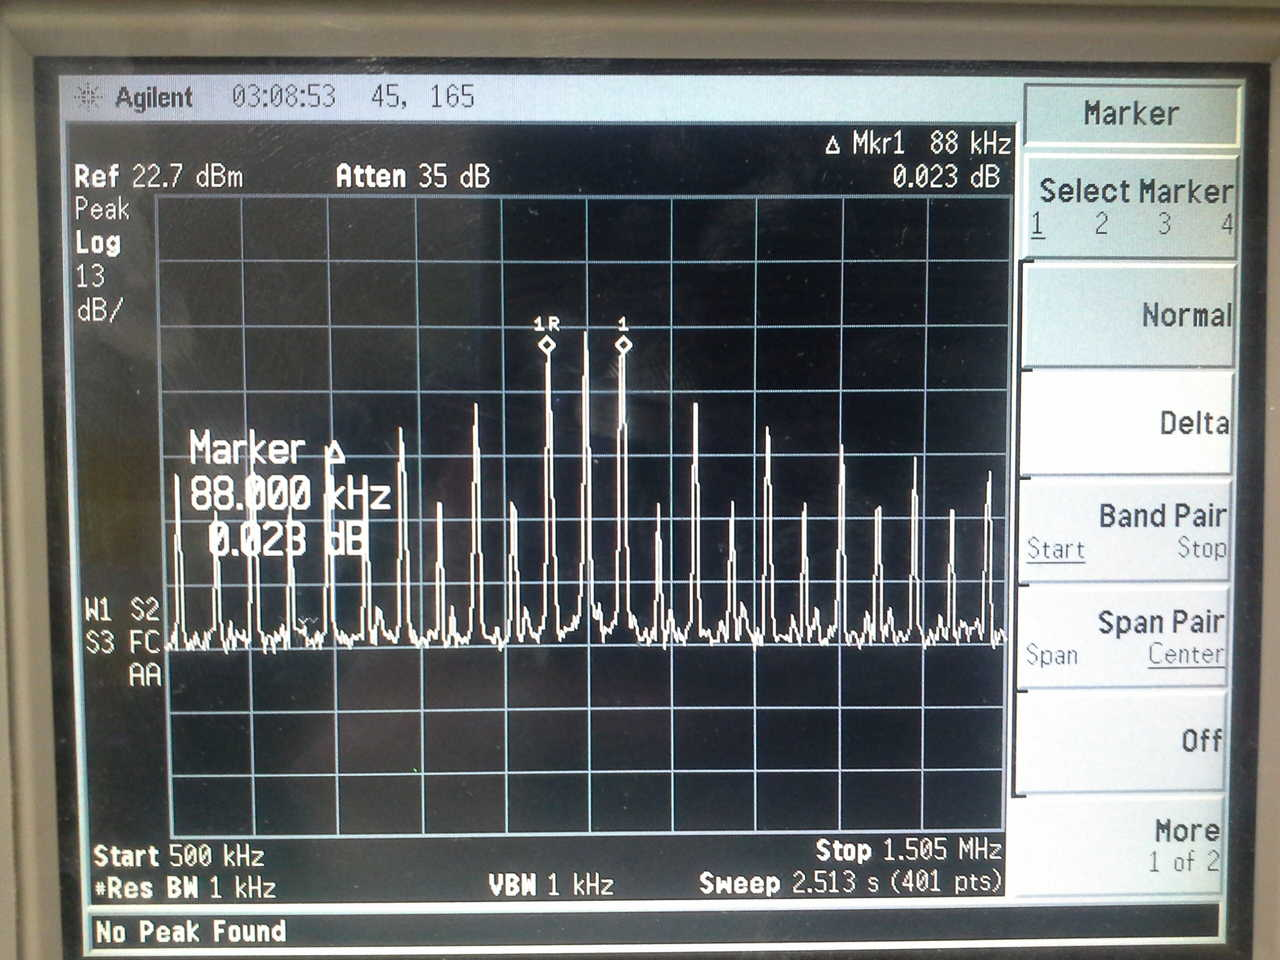
\includegraphics[scale=0.17]{../Grafiken/Frequenzspektrum_d_FreqModuliert_1.jpg}
		\caption{Frequenzdifferenz der ersten Seitenbänder\label{fig:frequenzspektrum_d_freqmoduliert_1}}
	\end{subfigure}%
	~
	\begin{subfigure}[t]{0.5\textwidth}
		\centering
		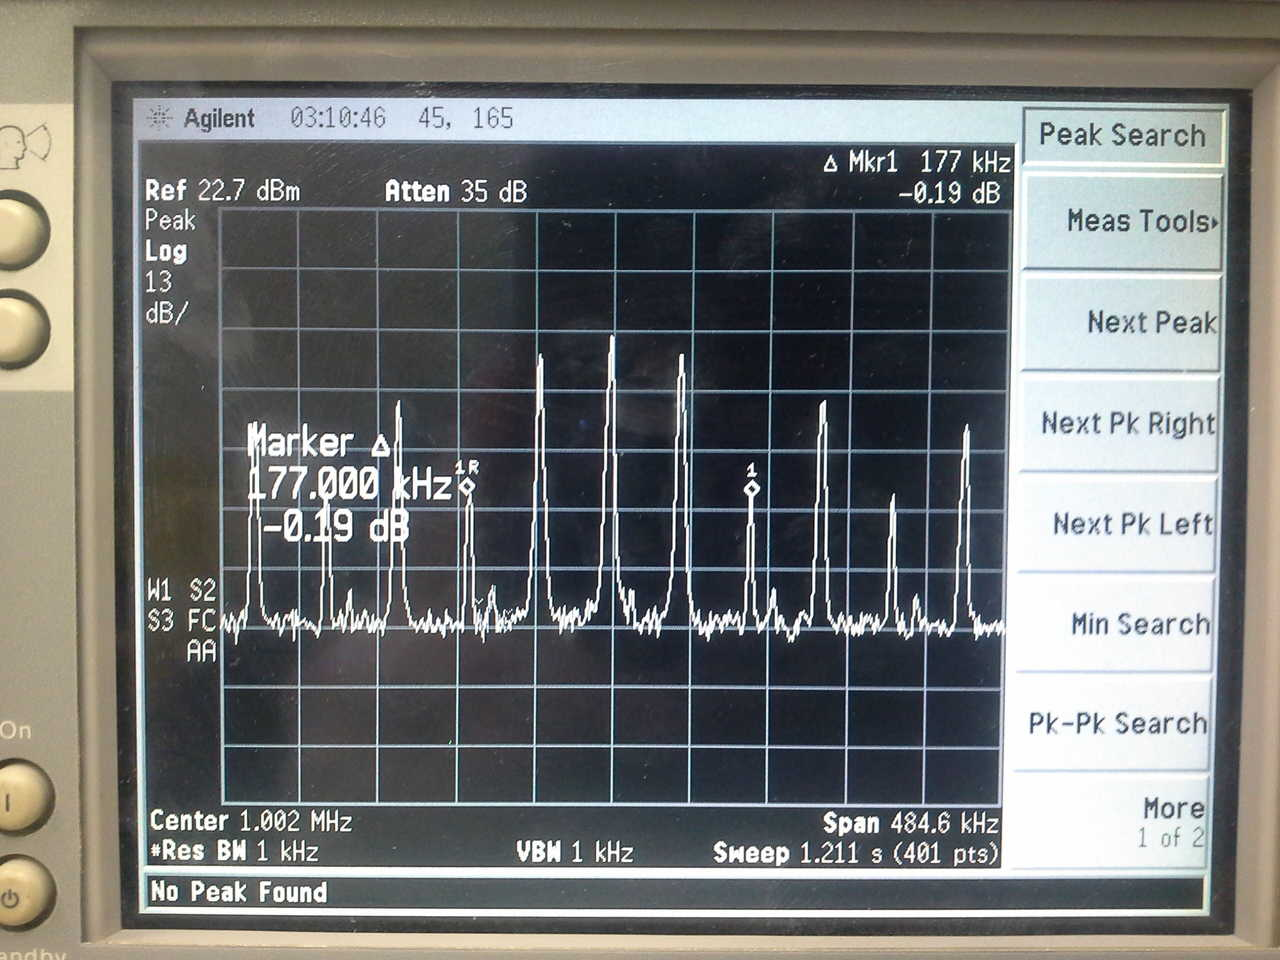
\includegraphics[scale=0.17]{../Grafiken/Frequenzspektrum_d_FreqModuliert_2.jpg}
		\caption{Frequenzdifferenz der zweiten Seitenbänder\label{fig:frequenzspektrum_d_freqmoduliert_2}}
	\end{subfigure}
	\caption{Frequenzspektrum der frequenzmodulierten Spannung. Hervorgehoben sind die Trägerfrequenz (a)
		und die Frequenzunterschiede der ersten (b)  und zweiten (c) Seitenbänder. 
		\label{fig:frequenzspektrum_d_freqmoduliert}}
\end{figure}
\FloatBarrier

Aus der in \cref{fig:frequenz_modulation_d_phasenvariation} dargestellten periodischen Phasenvariation
kann die maximale Frequenzvariation als Breite der abgebildeten \enquote{Verschmierung} bestimmt werden.

\FloatBarrier
\begin{figure}[!h]
	\centering
	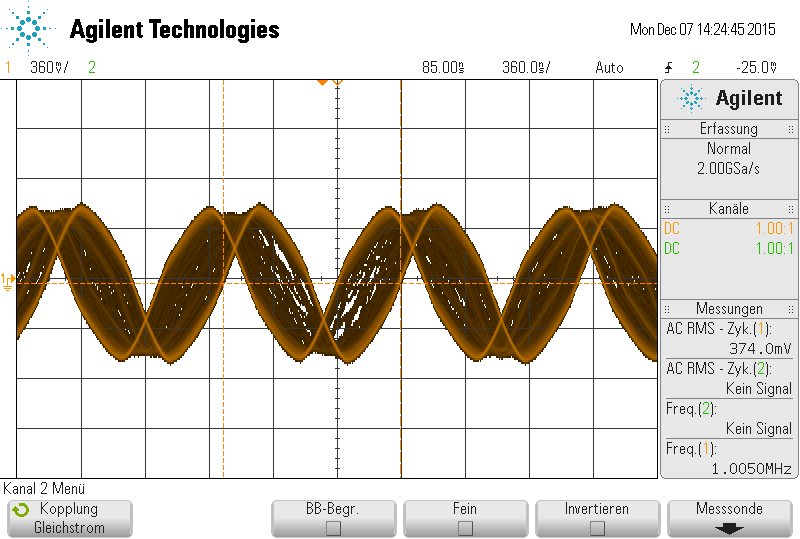
\includegraphics[scale=0.50]{../Grafiken/Messung_d2.png}
	\caption{Darstellung der periodischen Phasenvariation zwischen der modulierten Spannung und der
	Trägerspannung. Aus der Breite des dargestellten "verschmierten" Spannungsverlaufs, kann der Frequenzhub
	und der Modulationsgrad der Modulation bestimmt werden. \label{fig:frequenz_modulation_d_phasenvariation}}
\end{figure}
\FloatBarrier

Mit einer Kante im Ursprung und der anderen auf der ersten Einteilung in x-Richtung ergibt sich die 
Breite der Kurve aus der dargestellten Achseneinteilung zu 
\begin{empheq}{equation}
  \Delta x = \SI{360(10)}{\nano\second}.
\end{empheq}
Der angegebene Fehler stellt die geschätzte Ablesegenauigkeit aus der \cref{fig:frequenz_modulation_d_phasenvariation} dar.

Eine Periodendauer kann sowohl aus der selben Abbildung abgelesen werden
entspricht jedoch auch der Periodendauer der Trägerspannung 
\begin{empheq}{equation}
T_{\text{T}} = \SI{1000(1)}{ns}
\end{empheq}
mit der in \cref{eq:ausgangswerte_frequenz} angegebenen Frequenz $f_{\text{T}}$.
Aus dem Verhältnis der maximalen Verbreiterung $\Delta x$ und der Periodendauer ergibt sich nach 
Skalierung mit $2\pi$ der maximale Phasenhub
\begin{empheq}{equation}
 \Delta \varphi = 2\pi \cdot \frac{\Delta x}{T_{\text{T}}} = \SI{2.26(6)}{rad}.
\end{empheq}

Aus der formalen Darstellung einer frequenzmodulierten Spannung in \cref{eq:Frequenzmoduliert} 
ergibt sich der maximale Phasenhub für den Fall das $\cos\omega_\text{M}t = 1$ zu 
\begin{empheq}{equation}
\Delta \varphi = m \frac{f_{\text{T}}}{f_{\text{M}}}.
\end{empheq}

Damit und mit dem für den maximalen Phasenhub bestimmten Wert lässt sich der Modulationsgrad 
zu 
\begin{empheq}{equation}
m  = \num{0.097(4)}
\end{empheq}
berechnen. Aus diesem folgt über die \cref{eq:frequenzhub} der maximale Frequenzhub
\begin{empheq}{equation}
\Delta f = \SI{970(40)}{\kilo\hertz}.
\end{empheq}

Wie bereits das Frequenzspektrum \cref{fig:frequenzspektrum_d_freqmoduliert} vermuten ließ,
ist der Modulationsgrad dieser Spannung zwar kleiner eins, ist jedoch nicht gering im Sinne der Ungleichung $m\tfrac{\omega_{\text{T}}}{\omega_{\text{M}}} << 1$.

%Entsprechend folgt durch bilden des Kehrbruches die maximale Frequenzvariation und damit der Frequenzhub
%\begin{empheq}{equation}
%\Delta f = \frac{1}{\Delta t} = \SI{2.778}{\mega\hertz}.
%\end{empheq}
%
%Aus \cref{eq:frequenzhub} folgt damit der Modulationsgrad dieser frequenzmodulierten Spannung,
%\begin{empheq}{equation}
%	m = \num{2.778}.
%\end{empheq}
%Wie bereits das Frequenzspektrum \cref{fig:frequenzspektrum_d_freqmoduliert} vermuten ließ,
%ist der Modulationsgrad dieser Spannung nicht gering im Sinne der Ungleichung $m\tfrac{\omega_{\text{T}}}{\omega_{\text{M}}} << 1$.




\subsection{Demodulation von frequenzmodulierten Spannungen}

Die Demodulation der frequenzmodulierten Spannung aus \cref{sec:Frequenzmodulation} erfolgt
unter Verwendung eines Schwingkreises, der diese in eine Amplitudenmodulation überführt, und eines
Tiefpasses. Die Spannung die sich nach der Umwandlung in eine Amplitudenmodulation ergibt ist in 
\cref{fig:frequenz_moduliert_demodulation_amplitude} gezeigt. Die Spannung die an dem nachgeschalteten 
Tiefpass abgegriffen wird ist in \cref{fig:frequenz_moduliert_demodulation} dargestellt.



\FloatBarrier\begin{figure}[!h]
\centering
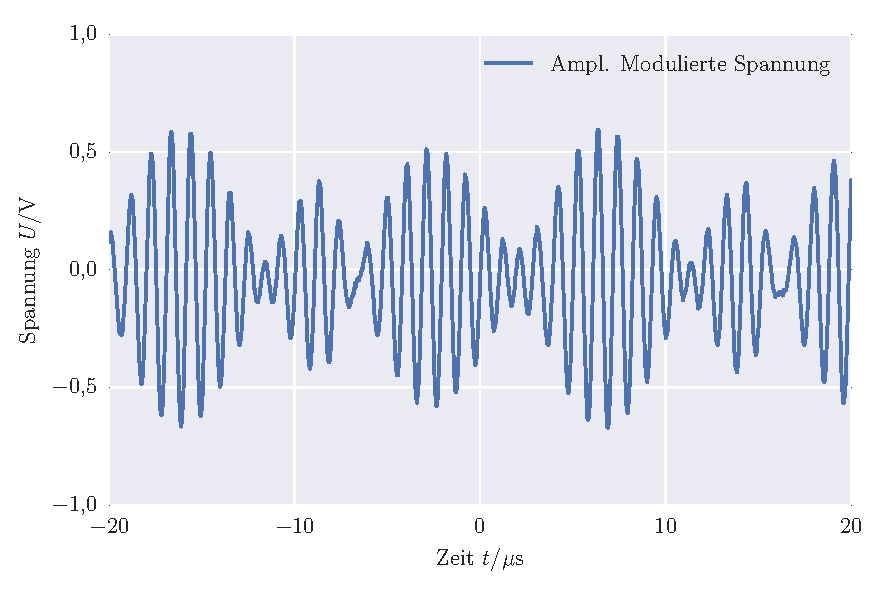
\includegraphics[scale=1]{../Grafiken/Frequenz_Moduliert_Demodulation_Amplitude.pdf}
\caption{Verlauf der amplitudenmodulierten Spannung nach Umwandlung der frequenzmodulierten Spannung durch
	einen Schwingkreis. Anhand des Abweichungen des Verlaufs von einer Schwebung ist zu erkennen, 
	dass weitere Frequenzen neben der Modulationsfrequenz zur Amplitudenmodulation beitragen.   \label{fig:frequenz_moduliert_demodulation_amplitude}}
\end{figure}
\FloatBarrier

\FloatBarrier\begin{figure}[!h]
\centering
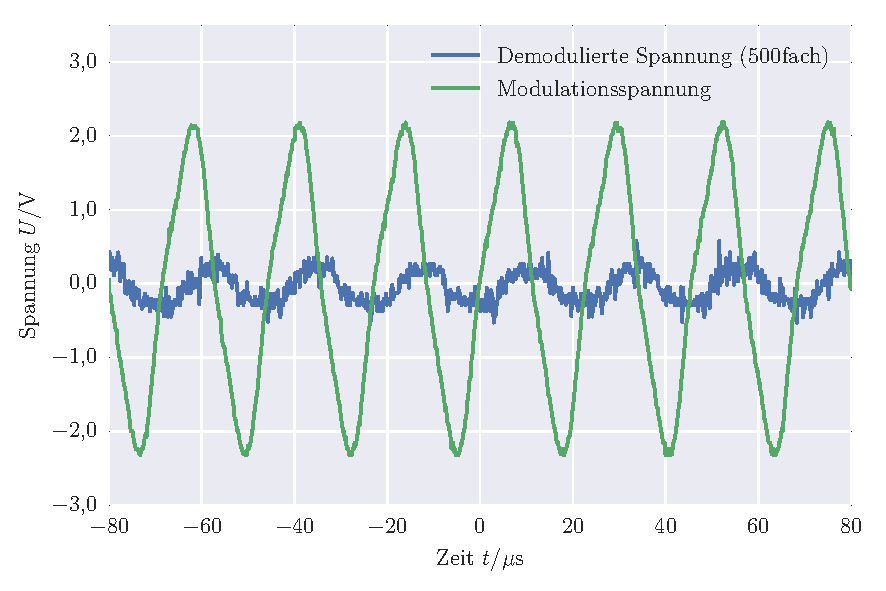
\includegraphics[scale=1]{../Grafiken/Frequenz_Moduliert_Demodulation.pdf}
\caption{\label{fig:frequenz_moduliert_demodulation}}
\end{figure}
\FloatBarrier

Der Verlauf der Amplitudenmodulation zeigt Abweichungen von dem einer Schwebung, der hier 
wie in \cref{fig:amplituden_modulierte_spannung_ohne_traeger} zu erwarten ist. Dies lässt auf eine ungenaue 
Einstellung des Schwingkreises schließen, wodurch weitere Frequenzen in der Amplitudenmodulation auftreten.
Die Spannung nach dem Tiefpass hat im Vergleich zur ursprünglichen Modulationsspannung eine sehr stark verringerte
Amplitude und die doppelte Frequenz. Die starke Dämpfung der Spannung ist auf die Widerstände der verwendeten 
Schaltung und die verwendete Bauteile, wie beispielsweise den Dioden im Ringmodulator, zurückzuführen. Der 
Unterschied in der Frequenz ist dadurch zu begründen, dass mit dem verwendeten 
Tiefpass alle Frequenzen über der doppelten Modulationsfrequenz unterdrückt wurden, deren auftreten wiederum durch 
die ungenaue Amplitudenmodulation begründet werden kann. Durch eine weitere Verringerung der Grenzfrequenz des
Tiefpasses konnte keine demodulierte Spannung mehr gemessen werden, da deren Amplitude mit diesen Einstellungen 
zu stark verringert wurde.